\chapter{Disseny del projecte}
En aquest capítol es plantejaran diferents aspectes relacionats amb la planificació i els requeriments del projecte.
%-----------------------------------------------------------------------
\section{Arquitectura}
Al projecte es pot observar l'arquitectura de tres capes, ja que compta amb un mòdul que fa de client o "frontend", un servidor o "backend" i una base de dades.
\begin{figure}[H]
    \centering
    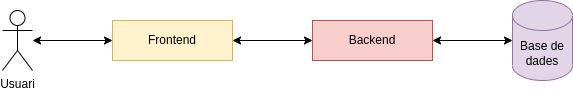
\includegraphics[width=\textwidth]{images/arquitectura.png}
    \caption{Arquitectura de tres capes}
    \label{fig:Arquitectura}
\end{figure}
%-----------------------------------------------------------------------
\section{Tecnologies}
\subsection{Codi font}
El frontend utilitza tecnologies web com HTML, CSS (Bootstrap), TypeScript o NodeJS, empaquetades amb Electron, i es comunica amb el backend mitjançant la llibreria Fetch i el protocol HTTP.
\\[3mm]
El backend es divideix en dos mòduls diferenciats:
\begin{enumerate}
    \item S'ha implementat una API Rest amb Java i el framework Spring Boot, aquest rep les peticions HTTP que el client envia als endpoints de la API i s'encarrega de processar-les i d'actuar com a intermediari amb la base de dades. D'aquesta forma mai es violarà l'arquitectura de tres capes.
    \item S'ha desenvolupat un mòdul que s'encarrega de la lògica del motor d'escacs i defineix el comportament i les normes del joc.
\end{enumerate}
\subsection{Base de dades}
La base de dades utilitza el motor H2 incrustat (“embedded”) i es comunica amb Spring Boot mitjançant la implementació del ORM Hibernate a Spring Data JPA.
\subsection{Entorn de desenvolupament}
Com a entorn integrat de desenvolupament s’utilitzarà IntelliJ IDEA.
\\[3mm]
Per al control de versions s’utilitzaran Git i GitHub, a més dels GitHub Workflows per a la integració, escalabilitat i testing del codi.
\\[3mm]
Per a facilitar el desenvolupament de la API, es realitzaran les peticions HTTP mitjançant Postman.
\subsection{Aspectes secundaris}
Es farà ús de GIMP i Inkscape per a l’edició d’imatges.
\\[3mm]
Els diagrames i esbossos es dissenyen amb la ferramenta  \href{https://app.diagrams.net/}{draw.io}
\\[3mm]
Per a escriure la documentació (aquest document) s’utilitzarà \LaTeX\ (LaTeX) i \href{https://www.overleaf.com/}{Overleaf}.

\begin{figure}[H]
    \centering
    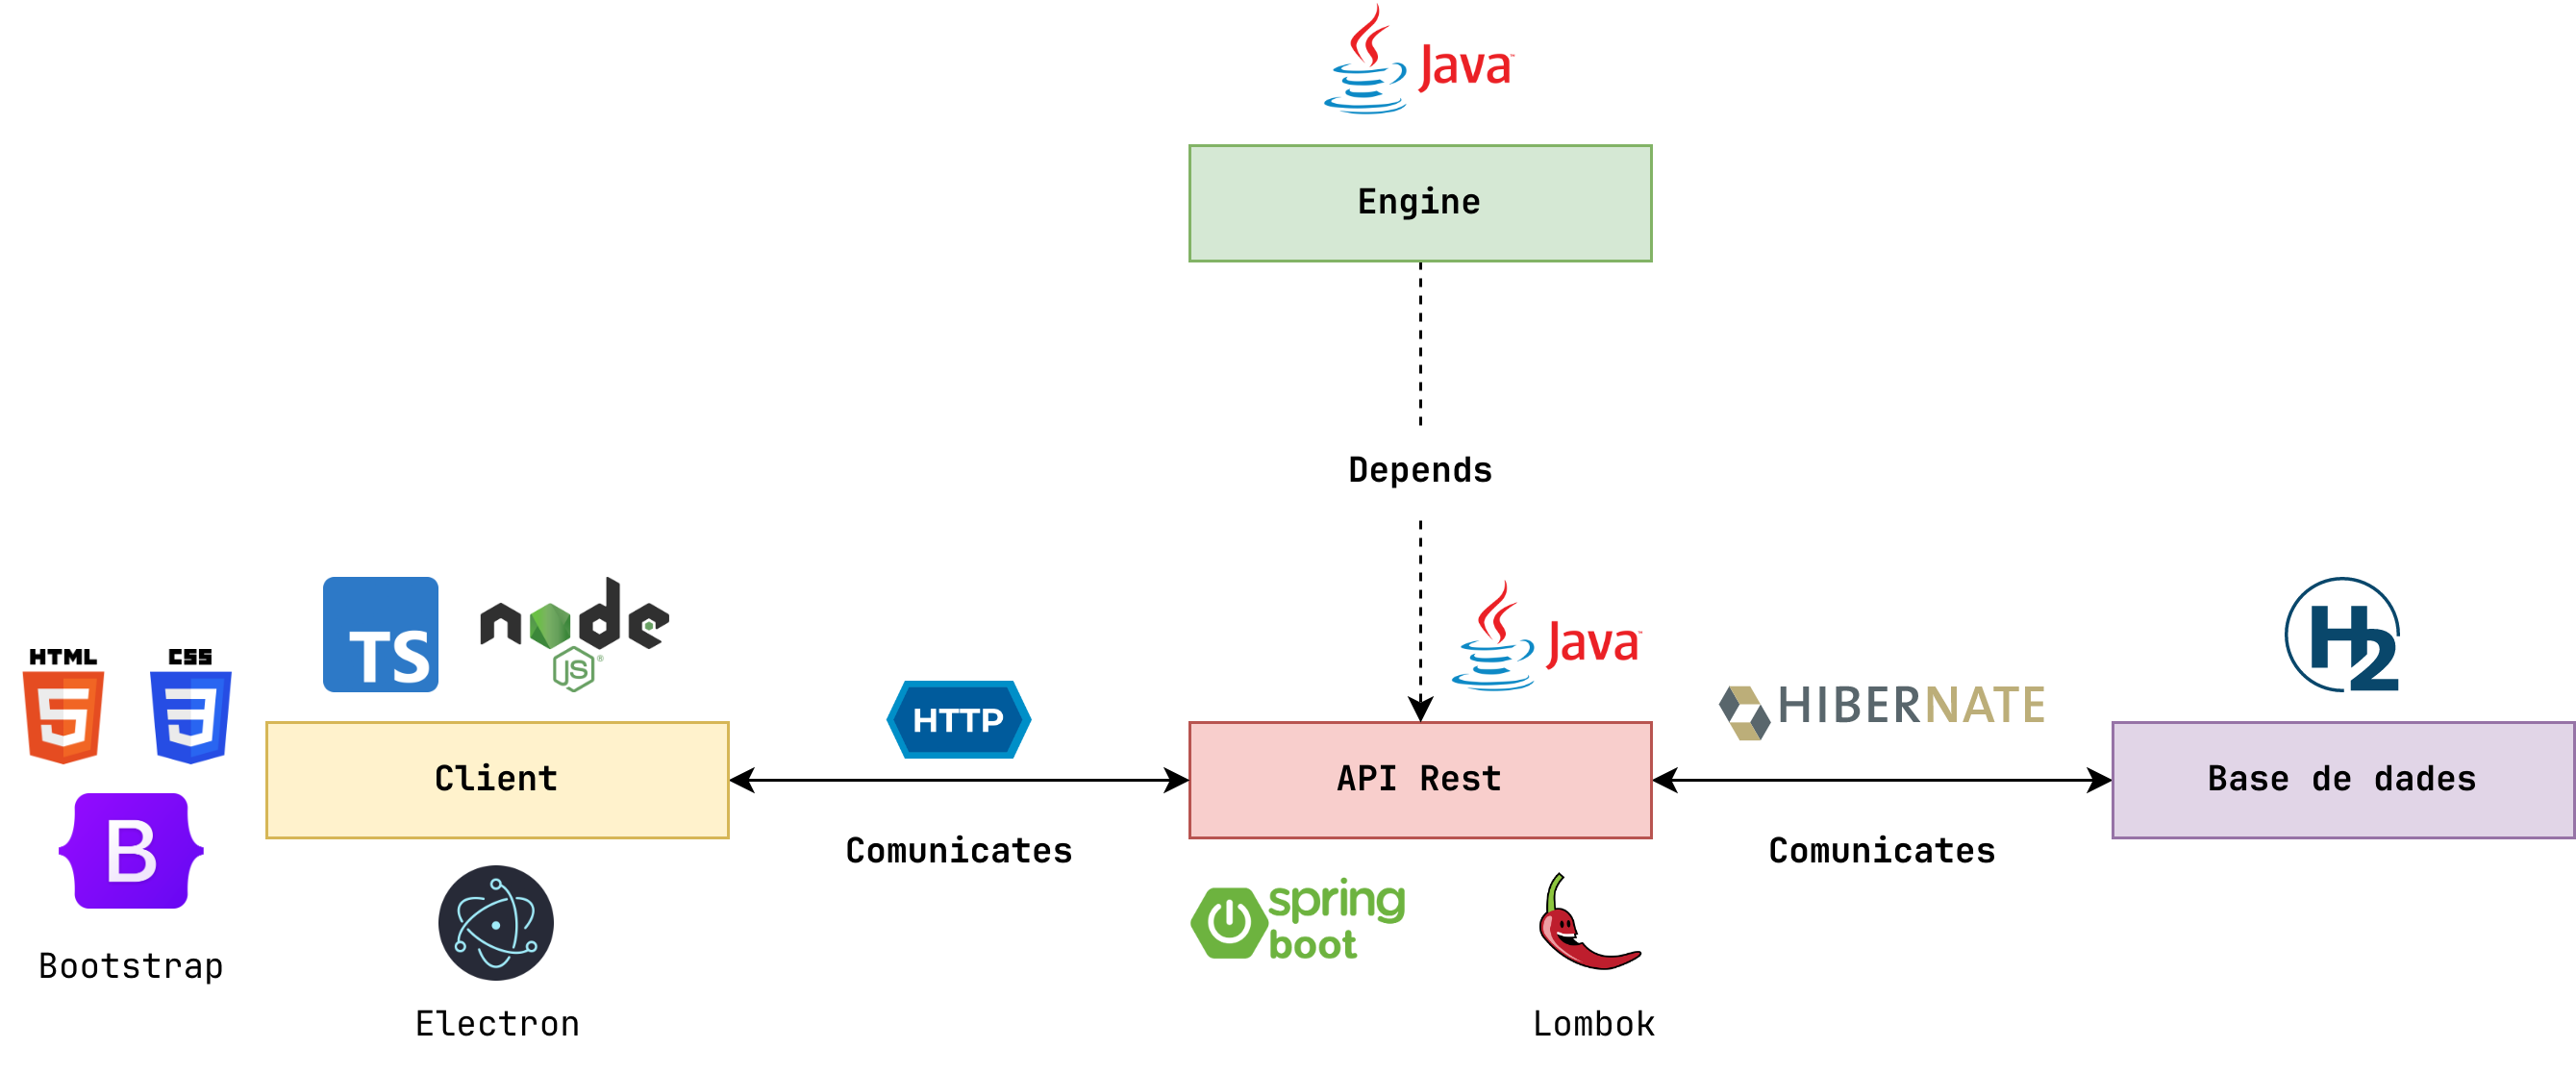
\includegraphics[width=\textwidth]{images/tecnologies.png}
    \caption{Tecnologies}
    \label{fig:Arquitectura}
\end{figure}
%-----------------------------------------------------------------------
\section{Requeriments}
\subsection{Sistema de registre}
Per a poder accedir a la aplicació els usuaris hauran de crear-se un compte introduint correu i contrasenya i assignar-se un nom d'usuari, les dades es validaran utilitzant Spring Validation i les credencials seran guardades de forma segura en la base de dades.
\subsection{Sistema d'inici de sessió}
Una vegada registrats, els usuaris hauran d’autenticar-se amb correu i contrasenya, aquestes dades es contrastaran amb les existents en la base de dades i se'ls permetrà o no l'accés.
\subsection{Sistema d'emparellament}
Una vegada autenticats, els usuaris tindran accés a la llista de jugadors i podran enviar i rebre sol·licituds de joc. 
\\[3mm]
Quan un usuari vol jugar amb altre, li envia una sol·licitud al destinatari, aquest podrà acceptar-la o rebutjar-la. Si decideix acceptar-la, els jugadors s'emparellaran a una nova partida.
\\[3mm]
Una vegada emparellats, els jugadors intercanviaran els missatges corresponents amb el servidor per a dur a terme la partida, fins la finalització d'aquesta.
\subsection{Implementació d’un “chess engine”}
\begin{wrapfigure}{r}{0.25\textwidth}
    \begin{center}
        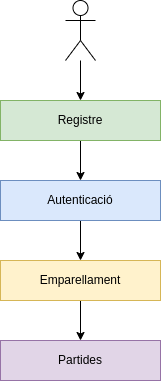
\includegraphics[width=0.75\linewidth]{images/multijugador.png} 
        \caption{Flux d'ús del programa}
        \label{fig:Flux d'ús del programa}
    \end{center}
\end{wrapfigure}
El motor d’escacs funciona com una “caixa negra” amb la que el servidor pot interactuar. El servidor executarà en aquest les jugades que rep dels clients, el motor les processarà i tornarà un estatus com a resposta, indicant el resultat d'aquesta execució.
\\[3mm]
Al joc trobem sis tipus de peces diferents que hereten d’una classe superior. La principal diferència entre aquestes es troba als tipus de moviments vàlids que poden realitzar, tenint en compte les normes del joc, s’han d’implementar aquests comportaments de forma individual per a cada peça.
\\[3mm]
Els moviments són la forma d’interactuar amb el motor, s'entén per moviment cadascuna de les jugades que s'executen al tauler.
Cal destacar que si un jugador realitza un moviment invàlid, no perdrà el torn, sinó que se li permetrà seguir fins que faça un vàlid. En aquest moment el torn passarà a l'oponent o s’acabarà la partida (si el moviment ocasiona l’estancament de la partida o l’escac i mat).
\\[3mm]
Els moviments estàndard o comuns a totes les peces són els de desplaçament i atac, encara que hi han altres moviments especials que només poden realitzar uns tipus de peces determinats, així com els moviments “matar al pas”, el bot inicial o la promoció al peó o l’enroc per al rei i la torre.
\subsection{Implementació d’una interfície gràfica d'usuari}
Per a codificar aquest apartat s'han utilitzat tecnologies web com HTML, CSS (Bootstrap), TypeScript o NodeJS, empaquetades amb Electron.
\\[3mm]
S'ha utilitzat HTML5 per a l'organització i el disseny estructural de les pàgines. HTML és un llenguatge de marcatge utilitzat per a crear i estructurar contingut en pàgines web. És l'estàndard per al desenvolupament web i proporciona una estructura bàsica per a organitzar elements en una pàgina. 
\\[3mm]
HTML utilitza etiquetes o tags per a marcar els diferents elements d'una pàgina web. Cada etiqueta té una funció específica i defineix com s'ha de mostrar o interpretar el contingut. Les etiquetes permeten crear encapçalaments, paràgrafs, llistes, taules, formularis, imatges, enllaços i molts altres elements que es poden trobar en una pàgina web. Aquestes etiquetes s'estructuren jeràrquicament, formant elements anidats que defineixen la relació i l'organització del contingut. A més, HTML també permet l'ús d'atributs en les etiquetes per a proporcionar informació addicional o personalitzar el comportament dels elements. 
\\[3mm]
En resum, HTML és el fonament de la web, ja que permet als desenvolupadors descriure i estructurar el contingut perquè els navegadors web puguin interpretar i mostrar les pàgines adequadament.
\\[3mm]
En quant al format i l'estil visual, Bootstrap ha segut un component imprescindible. Bootstrap és una biblioteca de codi obert que proporciona un conjunt de classes i estils predefinits per ajudar a desenvolupar interfícies web responsives de manera ràpida i senzilla. Aquesta biblioteca utilitza CSS per definir els estils i la presentació dels elements HTML, permetent als desenvolupadors estilitzar i estructurar els components de la seva pàgina web de manera coherent i consistent. Amb Bootstrap CSS, és possible aplicar estils comuns, com a mides de text, colors, marges, alineacions i respostes a diferents dispositius, amb facilitat. Això permet crear un disseny visualment atractiu i professional, amb una experiència de l'usuari optimitzada en diferents plataformes i resolucions de pantalla. No obstant, s'ha escrit codi CSS addicional quan era necessari.
\\[3mm]
S'ha optat per utilitzar el llenguatge TypeScript per a la part lògica i interactiva del projecte. TypeScript és un llenguatge de programació de codi obert que amplia la sintaxi de JavaScript. Aquest llenguatge proporciona funcionalitats addicionals com ara tipat estàtic, orientació a objectes i suport per a característiques modernes de JavaScript.
\\[3mm]
El tipat estàtic és una característica clau de TypeScript que permet declarar i assignar tipus de dades a les variables, paràmetres de funcions i retorn de valors, entre d'altres. Això ajuda a detectar errors de tipus durant el desenvolupament, millorant la robustesa i la escalabilitat del codi.
\\[3mm]
A més, TypeScript facilita la programació orientada a objectes, permetent la creació de classes, herència, interfícies i altres conceptes propis de la programació orientada a objectes. Aquesta organització estructurada del codi ajuda a millorar la seva claredat i reutilització.
\\[3mm]
A més TypeScript també proporciona suport per a les funcionalitats més modernes de JavaScript, com ara els mòduls ES6, les funcions de fletxa i altres característiques sintàctiques avançades.
\\[3mm]
Per a realitzar i rebre peticions HTTP s'ha utilitzat l'API Fetch. És una interfície proporcionada per JavaScript que permet realitzar peticions HTTP asíncrones a un servidor i obtenir les respostes en format de Promises. L'API Fetch és compatible amb els formats de dades comuns, com ara JSON, i permet realitzar operacions addicionals, com ara afegir interceptors per manipular les peticions i respostes abans que siguin processades o afegir opcions personalitzades, com capçaleres i dades en el cos de la petició.
\subsection{Persistència de dades rellevants a les partides}
Les credencials dels usuaris i la informació de les partides es guarden a una base de dades implementada amb H2. S'ha triat aquest sistema gestor de base de dades per la seua senzilla integració amb Spring Boot, ja que no requereix cap configuració per a fer-lo funcionar.
\\[3mm]
Cada partida ha de tindre un identificador únic i estar relacionada amb dos jugadors, enllaçats a aquesta s’agruparan els moviments realitzats amb format “Portable Game Notation”.
\\[3mm]
Per a l'emmagatzemament de dades, s'ha utilitzat la implementació del ORM Hibernate proporcionada per Spring Data JPA. Spring Data JPA té com a objectiu simplificar l'accés i la interacció amb bases de dades en aplicacions Java. Proporciona una capa d'abstracció d'alt nivell sobre l'API de Persistència de Java (JPA), que és una especificació per a frameworks d'ORM (Mapeig Objecte-Relacional) en Java.
\\[3mm]
Spring Data JPA combina el poder de Spring Boot i JPA per oferir als desenvolupadors una manera simplificada de treballar amb bases de dades relacionals. Elimina la necessitat d'escriure codi boilerplate per a operacions comunes de bases de dades, com ara operacions CRUD (Crear, Llegir, Actualitzar, Esborrar), creació de consultes i gestió de transaccions.
\\[3mm]
Amb Spring Data JPA, pots definir repositoris que encapsulen les operacions de bases de dades en entitats. Seguint determinades convencions de nomenclatura o utilitzant consultes personalitzades, pots generar automàticament consultes SQL per a operacions comunes sense haver d'escriure declaracions SQL explícites. Això redueix considerablement la quantitat de codi que cal escriure i millora la productivitat de desenvolupament.
\\[3mm]
Utilitzant Spring Data JPA, pots aprofitar els avantatges de JPA i els conceptes d'ORM, alhora que beneficies de les funcionalitats i convencions proporcionades per Spring Data. Simplifica l'accés a bases de dades, fomenta la reutilització de codi i ajuda els desenvolupadors a centrar-se en la lògica de negoci en lloc de les interaccions de baix nivell amb la base de dades.
%-----------------------------------------------------------------------
\section{Esbós de la interfície gràfica}
\subsection{Formularis d'inici de sessió i registre}
\begin{figure}[H]
    \centering
    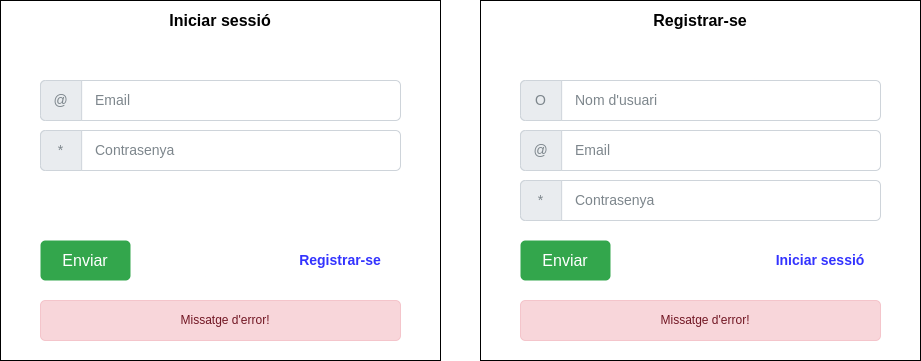
\includegraphics[width=\textwidth]{images/login.png}
    \caption{Esbós dels formularis d'inici de sessió i registre}
    \label{fig:Esbós dels formularis d'inici de sessió i registre}
\end{figure}
\subsection{Pàgina principal}
\begin{figure}[H]
    \centering
    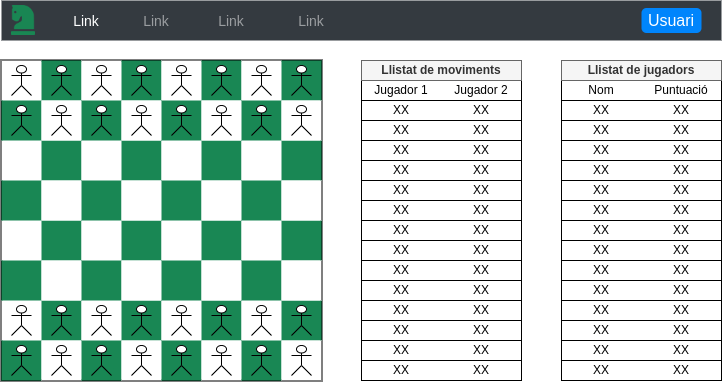
\includegraphics[width=\textwidth]{images/index.png}
    \caption{Pàgina principal}
    \label{fig:Pàgina principal}
\end{figure}
%-----------------------------------------------------------------------
\section{Base de dades}
La base de dades contindrà quatre entitats: jugadors, moviments, partides i sol·licituds de joc.
\\[3mm]
Dels jugadors volem guardar el seu nom d'usuari, el seu correu, la seua contrasenya encriptada i la seua puntuació. El nom i la puntuació seran visibles per a la resta d’usuaris. El correu i la contrasenya s’utilitzaran per a autenticar-se.
\\[3mm]
En quant als moviments és important saber el valor d'aquests, que s’almacenarà amb format “Portable Game Notation”, així com quin ha segut el seu efecte o estatus a la partida. A més hem de relacionar-los amb el jugador que l'ha realitzat i la partida on s'ha executat.
\\[3mm]
A la taula partides es guardarà la sol·licitud de joc amb la que han accedit els usuaris (d'aquesta manera es poden relacionar els usuaris participants amb la partida), també guardarem qui ha segut el guanyador i si la partida ha acabat o escara està sent jugada.
\\[3mm]
Les sol·licituds de joc són un element més bé temporal, ja que deixen de ser vàlides una vegada s'accepten, es rebutgen o expiren.
En aquesta tabla es interessant almacenar l'hora de creació i d'expiració, també l'estat de la sol·licitud i els usuaris involucrats en aquesta.
\begin{figure}[H]
    \centering
    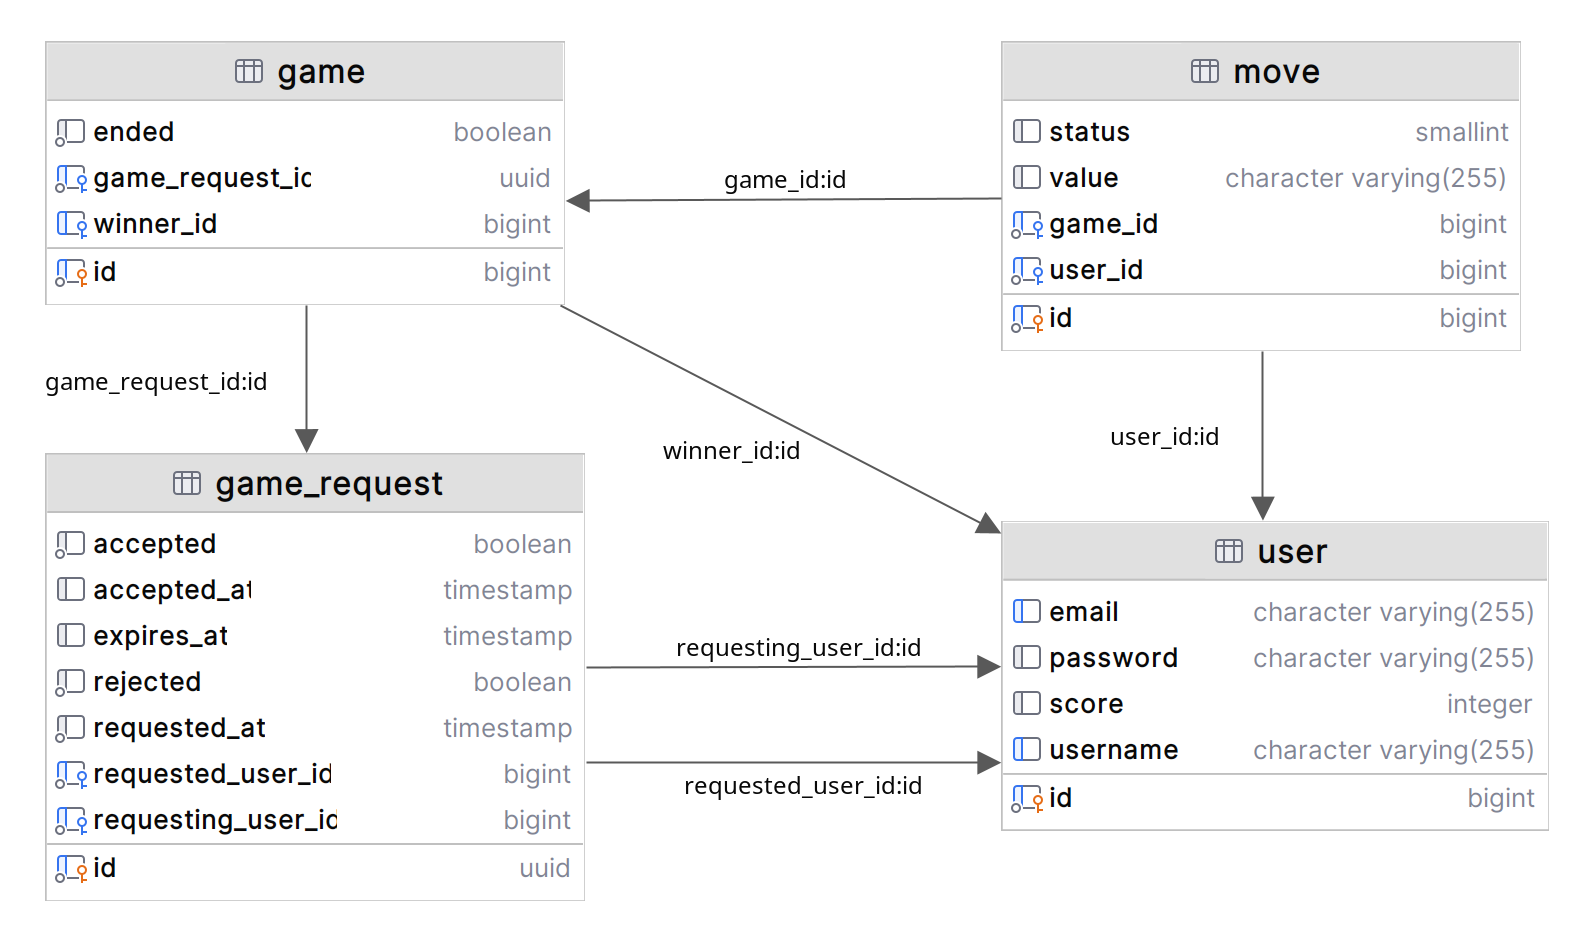
\includegraphics[width=\textwidth]{images/entitat-relacio.png}
    \caption{Diagrama entitat relació}
    \label{fig:Diagrama entitat relació}
\end{figure}